
% this file is called up by thesis.tex
% content in this file will be fed into the main document

%: ----------------------- introduction file header -----------------------
\chapter{Experiments}\label{ch:experiments}

\graphicspath{{experiments/figures/}}

% -------------------------------------------------------------
% -- Experiments
% -------------------------------------------------------------

The hypotheses raised in this thesis have been further validated in real projects. The implementation of the proposed algorithms and their execution in systems used by third parties, has allowed us to verify the results obtained during the evaluations. Some of these projects are framed in the health field, specifically in the area of HIV treatment (Section \ref{sec:polypharmacy}) and, recently, in the field of COVID-19 treatment (Section \ref{sec:drugs4covid}). In both cases our algorithms have helped to analyze the use of drugs to treat diseases. There are also projects aimed at measuring the impact of scientific research, at a national level through the creation of patents and research collaborations (Section \ref{sec:corpus-viewer}), and by research area from a point of view of originality and creativity of research (Section \ref{sec:drinventor}). Finally, the results of this thesis have also been used to facilitate the exploration of public procurement data in Europe (Section \ref{sec:tbfy}). Tenders performed by public administrations across Europe were related in an automatic and language-independent way to facilitate their exploration and allow local administrations to know how similar processes are managed in other countries.  

\section{DrInventor}
\label{sec:drinventor}

Scientific creativity and innovation are key concepts at a time of rapid technological change. Technologies have great potential to supplement human ingenuity in science by overcoming the limitations that people suffer in pursuing scientific discovery. DrInventor\footnote{\url{http://drinventor.eu}} proposes an original system to provide inspiration for scientific creativity by utilizing the rich presence of web-based research resources \citep{Dong2017DrIP}. It is like a personal research assistant that informs researchers of a broad spectrum of relevant research concepts and approaches, by assessing the novelty of research ideas, and by offering suggestions of new concepts and workflows with unexpected features for new scientific discovery.

Our topic modeling framework, librAIry (more details in Chapter \ref{ch:scalability}), and the topic-based characterization to measure the similarity between documents (described in Section \ref{sec:topicmodel}) powered the DrInventor platform to automatically relate scientific publications from their content. We created a harvester module\footnote{\url{https://github.com/cbadenes/camel-oaipmh}} (Section \ref{sec:librairy-modules})  that was able to ingest and index research resources from external sources based on the Open Archive Initiative Protocol for Metadata Harvesting\footnote{\url{https://www.openarchives.org/pmh/}}. The resources were processed at different levels of granularity: from the entire documents, to their individual items, parts or even individual words contained in them. On top of those resources DRInventor attaches different annotations that further described the instances and gave support to different operations leveraging on them. The model (Figure \ref{fig:drinventor-model}) provided a standard way of representing research documents, and was flexible enough to give support to a great variety of analysis techniques bringing value to the information stored in it. 

\begin{figure}[ht]
    \centering
    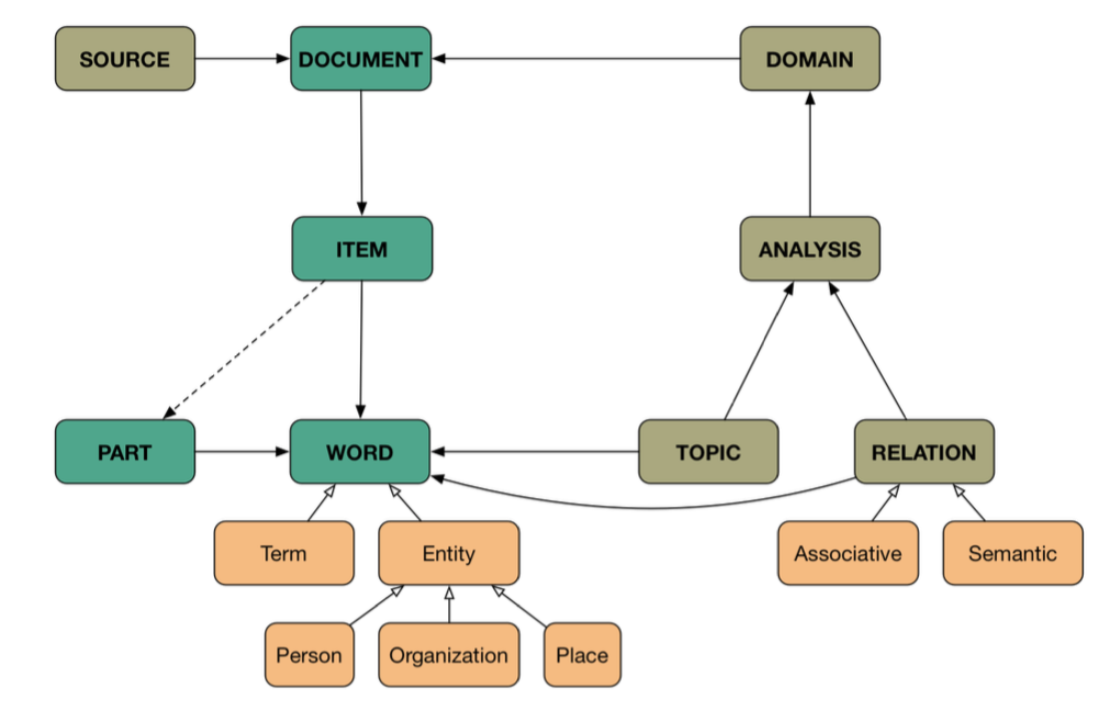
\includegraphics[width=0.8\linewidth]{drinventor-model.png}
    \caption{Overview of Resources in DRInventor Platform}
    \label{fig:drinventor-model}
\end{figure}


The main types of resources that were considered in DRInventor, from the most fine/grained to the most general ones, were:
\begin{itemize}
\item \textbf{Word}: a meaningful element of writing inside a document, composed by a sequence of characters.
\item \textbf{Part}: logical division of a document, based on categories of the research discourse such as abstract, introduction, methods, results, conclusions, etc., including also the types of rhetorical sentences \citep{Ronzano2015} (i.e. approach, background, challenge, future work or outcomes).
\item \textbf{Item}: element that make up a research object such as a paper, programming-code, an image, a workflow, and so on.
\item \textbf{Document}: aggregation of \textit{items} that composes a research object.
\item \textbf{Source}: repository where research objects are located. It is used from the platform to automatically retrieve resources.
\item \textbf{Domain}: collection of resources created after ingesting the research objects from a repository specified by a \textit{source}.
\item \textbf{Analysis}: execution of an algorithm over a particular \textit{domain} in the platform. It is responsible for the creation of annotations, such as \textit{topics} and \textit{relations}.
\item \textbf{Term}: concepts results of the execution of different Natural Language Processing algorithms.
\item \textbf{Entity}: named entities such as person, location, or organization.
\item \textbf{Topic}: subject that the corpus is elaborating on, such as research areas or trending issues in scientific domain.
\item \textbf{Relation}: associative or semantic connection between two resources in a \textit{domain}.
\end{itemize}

The DrInventor model served us to refine the model proposed in this thesis (see Section \ref{sec:representing-corpora}). Some resources have not been addressed (e.g. \textit{Source}, \textit{analysis}, \textit{topic} and \textit{relation}) to minimize the representation elements to those that can be used to create probabilistic topic models and to calculate similarities between documents (e.g. document, domain, annotation). It has also allowed us to generalize our model by adding a \textit{snippet} resource to represent any element (e.g. part, sentence, entity) that may appears in a document.


\section{Corpus Viewer}
\label{sec:corpus-viewer}
...


\section{Polypharmacy and Drug-drug Interactions}
\label{sec:polypharmacy}

Does the number of concomitant drugs in people living with Human Immunodeficiency Virus (HIV) increase with age and is it greater than in non-HIV-infected persons? This research question \citep{Badenes-Olmedo2019c} seems to be far from the scope of this thesis. However, if we take into account that  concomitant drugs are the drugs that a patient also uses to treat other diseases, we can draw an analogy to bring it closer to our domain. It aims to analyze patients from the medicines they receive, and our algorithm organizes documents described by topics. A patient, seen as a document, is described by the drugs he/she receives to treat HIV, which can be represented as topics, and the drugs he/she receives to treat other diseases (i.e concomitant drugs) , which would be used to set the relevance of each topic from their interactions. The relationships between patients depend on the drugs they share, and can be measured by the topics they share when they are represented as documents.


\begin{figure}[ht]
    \centering
    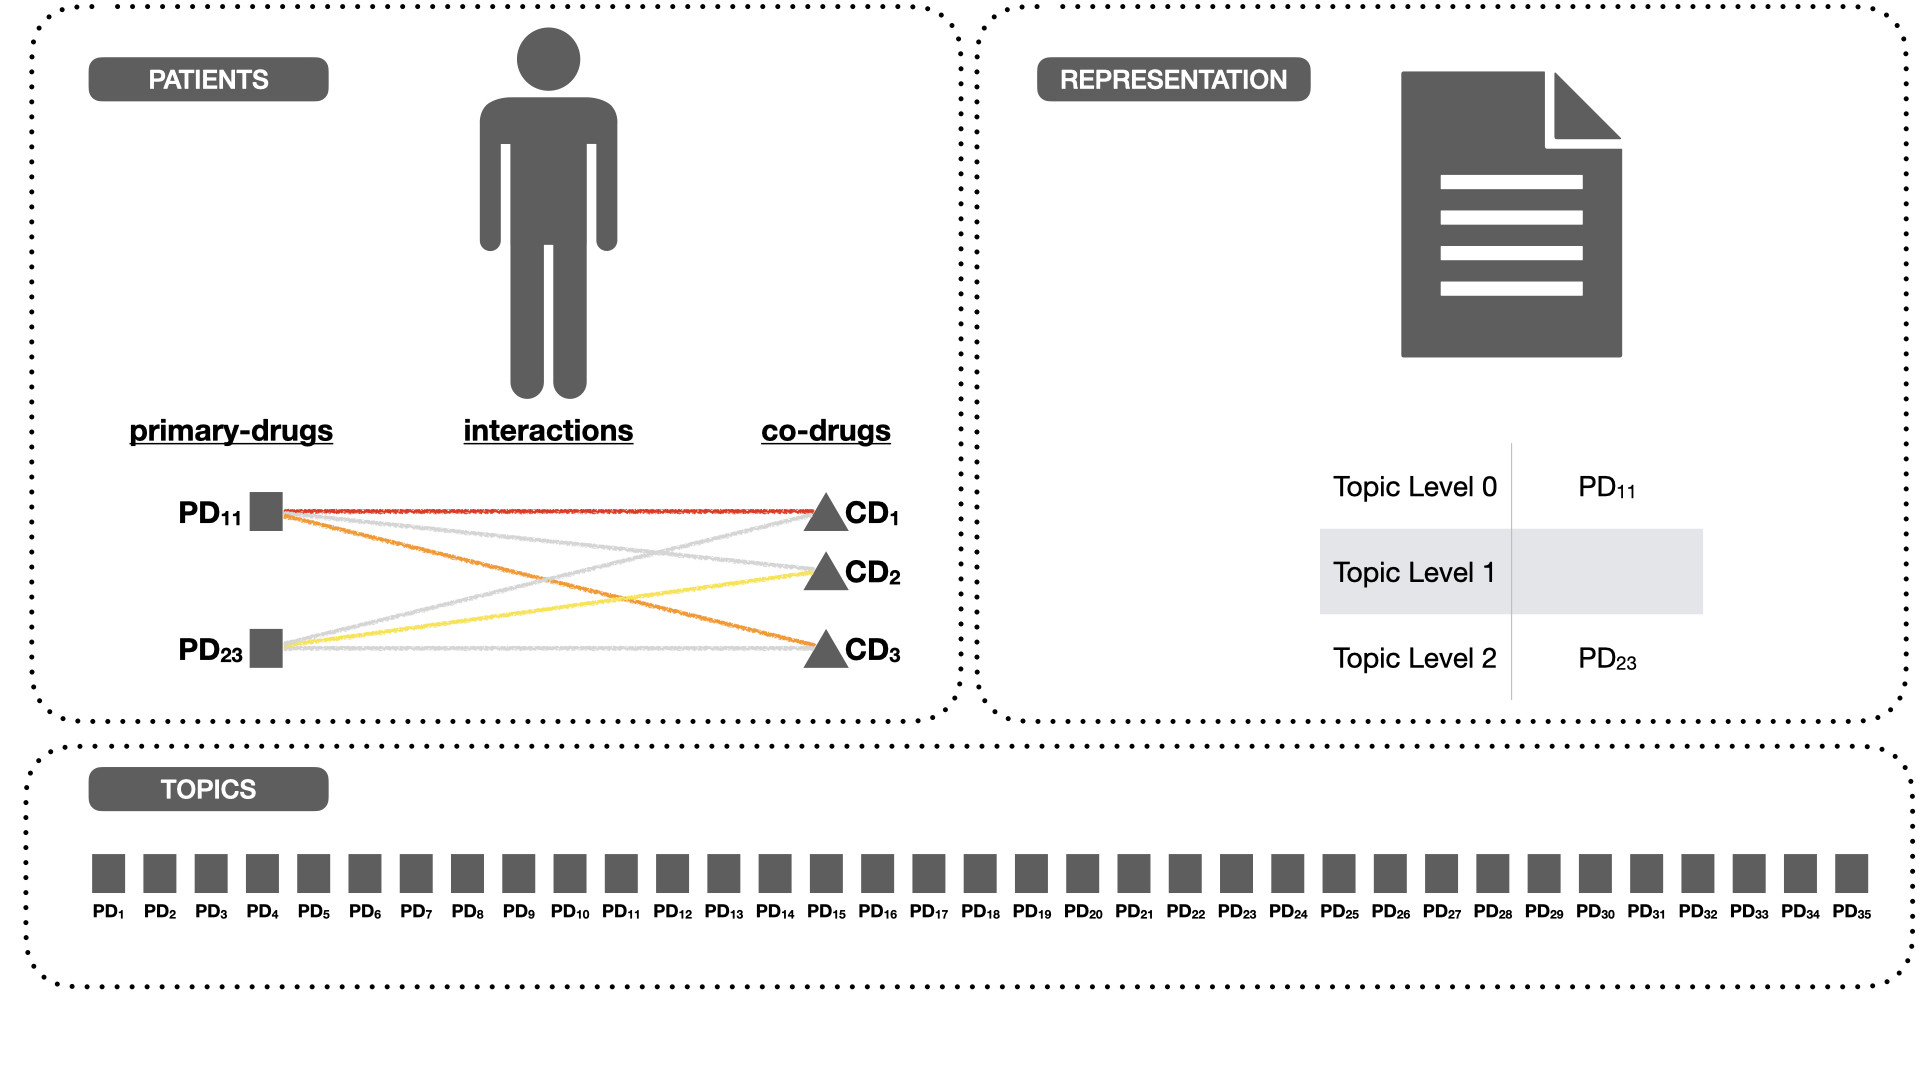
\includegraphics[width=0.7\linewidth]{polypharmacy.png}
    \caption{Representation of patients through topic hierarchies based on the interactions between primary-drugs and co-drugs}
    \label{fig:polypharmacy-topics}
\end{figure}

Specifically, in this work we were able to put into practice our approach to make comparisons (Chapter \ref{ch:comparisons}) when discovering drug–drug interactions (DDIs) in HIV patients. The anonymized registries from the Madrid Health Service (SERMAS) database were used to build a working database with information about all patients who picked up antiretrovirals (ARVs) or non-HIV medications during the study period. A total of 22,945 people living with HIV and 6,613,506 individuals without HIV had received medications. Medications from the SERMAS database were separated into ARVs and non-HIV drugs: 35 primary-drugs (i.e ARVs medications) and 1,058 co-drugs (i.e non-HIV medications). All drug pairs between primary- and co-drugs were interrogated using the University of Liverpool (UoL) Drug Interactions Database\footnote{\url{https://www.hiv-druginteractions.org}}, with more than 24,000 HIV DDIs between ARVs and non-HIV medications, to generate a comprehensive list of potential DDIs. The Liverpool flag classification  categorizes the severity of DDIs as follows: a red flag indicates medications that should not be coadministered as they might lead to serious adverse events or profoundly affect antiretroviral therapy efficacy; an orange flag indicates a potential interaction that might require dosage modification or close monitoring to minimize clinical consequences; a yellow flag indicates a potential interaction of weak relevance not requiring additional monitoring or dosage adjustment; a green flag indicates no anticipated risk of inter-action; and a gray flag indicates no clear data are available to assess whether a DDI will occur.

We built a representation system where each primary-drug was represented as a topic, and each patient was described as a document containing those topics with different weights (Figure \ref{fig:polypharmacy-topics}). This value depends on the DDIs between the primary-drugs and the co-drugs of the patients. Red-flag interactions correspond to the most relevant topics (i.e. level 0), orange-flag interactions correspond to the following topics (i.e. level 1), and yellow-flag interactions correspond to the least relevant topics (i.e. level 2). Primary-drugs are assigned to the most relevant level. Patients are thus described by DDIs, making it easy to identify sets of risks according to the severity of the interactions.


\begin{figure}[ht]\centering
   \begin{minipage}{0.49\textwidth}
     \frame{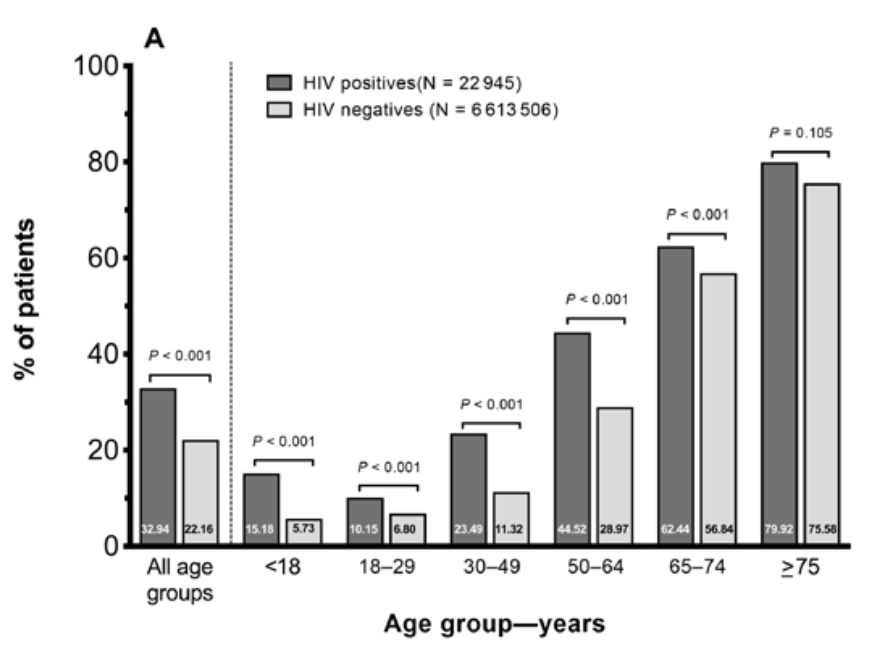
\includegraphics[width=\linewidth]{polypharmacy01.png}}
     \caption{Patients grouped by age}\label{subfig:poly-age}
   \end{minipage}
   \begin {minipage}[c]{0.49\textwidth}
     \frame{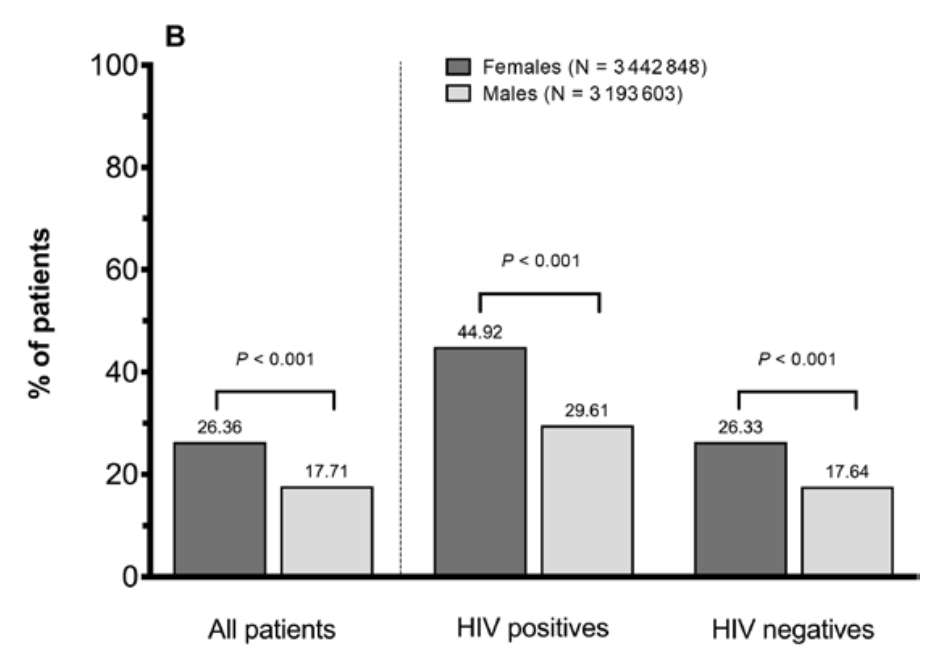
\includegraphics[width=\linewidth]{polypharmacy02.png}}
     \caption{Patients grouped by gender}\label{subfig:poly-gender}
   \end{minipage}
   \caption{Distribution of polypharmacy among people living with and without HIV according to age and gender \citep{Badenes-Olmedo2019c}.}
   \label{fig:polypharmacy}
\end{figure}

Our contribution facilitates the analysis of patients and drugs (interactions) without having to make all the comparisons between them (Figure \ref{fig:polypharmacy}). Patients are grouped by interactions on the same primary medications. The source code we have developed to discover drug interactions is publicly available for reuse\footnote{\url{https://github.com/cbadenes/hiv-ichart-client}}, but for privacy reasons we cannot publish the code to manage patients. 

\section{TheyBuyForYou}
\label{sec:tbfy}

In order to improve public procurement in European Union (UE), TheyBuyForYou \citep{Ahmet2020} aimed to provide high quality, open, and integrated procurement data. The lack of common agreement across the EU on the data formats for exposing such data sources and on the data models for representing such data, leads to a highly heterogeneous technical landscape. In this context, a knowledge graph (KG) based platform and end-users tools have been created and publicly released for integrating and reconciling cross-border and cross-language procurement and company data. But procurement processes are not only creating structured data, but also constantly creating additional documents (tender specifications, contract clauses, etc.). These are commonly published in the official language of the corresponding public administrations. Only some of these, for instance those published in TED\footnote{\url{https://ted.europa.eu}}, are multilingual, but the documents in the local language are typically longer and much more detailed than their translations into other languages.

A civil servant working at a public administration on a contracting process may be interested in understanding how other public administrations in the same country or in different countries (and with different languages) have worked on similar contexts. Examples may include finding organizations related to a particular procurement process, or search for tenders related to given
procurement text. Based on our results to create language-independent probabilistic topic models (Chapter \ref{ch:multilinguality}), we worked on an cross-lingual search engine\footnote{\url{tbfy.librairy.linkeddata.es/search-api}} that provides support to these types of users, with the possibility of finding documents that are similar to a given one independently of the language in which it is made available (Figure \ref{fig:tbfy-architecture}). We also created a Jupyter notebook with some representative examples to facilitate its use\footnote{\url{http://bit.ly/tbfy-search-demo}}.

\begin{figure}[ht]
    \centering
    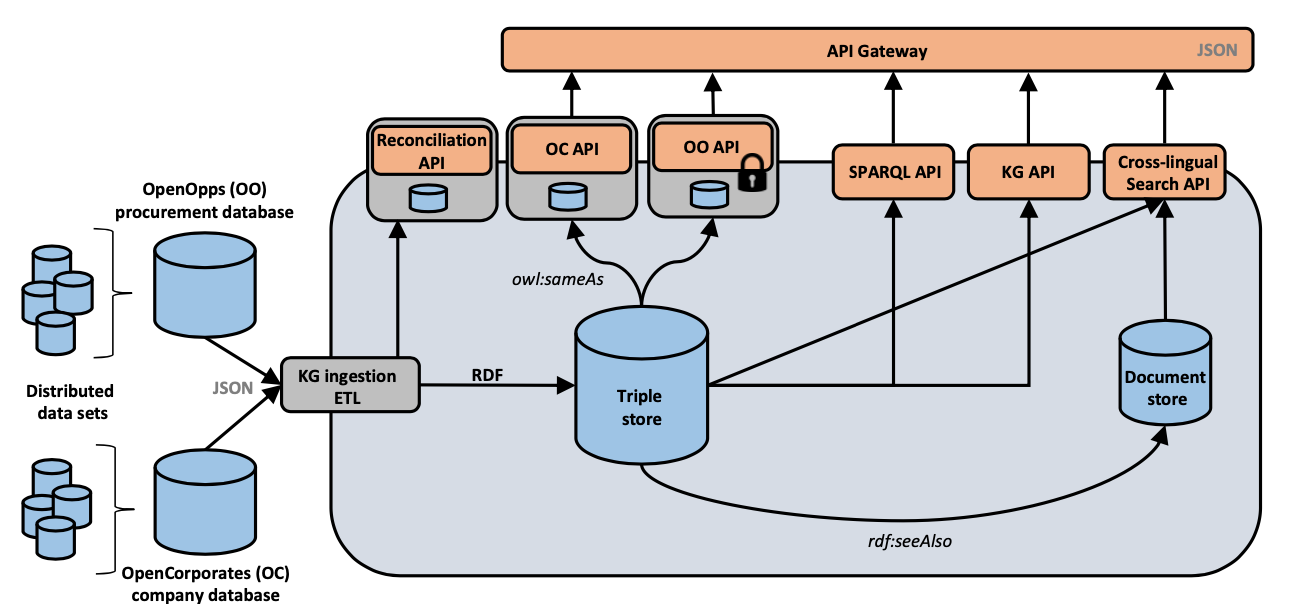
\includegraphics[width=0.7\linewidth]{tbfy-architecture.png}
    \caption{High-level architecture of the TheyBuyForYou platform}
    \label{fig:tbfy-architecture}
\end{figure}

The document search engine is based on the use of cross-lingual labels created from sets of cognitive synonyms (synsets) and unsupervised probabilistic topic models. The original low-dimensional latent space created by probabilistic topic models \cite{Badenes-Olmedo2019a} was extended with two new languages. In addition to the original English, French and Spanish models, we created Portuguese and Italian models to increase the common space shared by all languages (see Section \ref{sec:crosslingual-models}). Topics were described by cross-lingual labels created from the list of concepts retrieved from the Open Multilingual WordNet. Each word was queried to retrieve its synsets. The final set of synsets for a topic was the union of the synsets from the individual top-words of a topic. Documents were then represented as data points and transformed from the original feature space based on mono-lingual topic distributions into a cross-lingual hierarchical-based space, so that similar data points share relevant cross-lingual concepts (see Figure~\ref{fig:topic_models}). Since topic models create latent themes from word co-occurrence statistics in a corpus, a cross-lingual topic specifies the knowledge about the word-word relations it contains for each language. 

The data and platform components were made available openly for the community to contribute and use; a catalogue is available online\footnote{\url{https://tbfy.github.io/platform}} with pointers to the code repositories, online versions of the artefacts, and relevant documentation


\section{Drugs4Covid}
\label{sec:drugs4covid}

In the absence of sufficient medication for COVID patients due to the increased demand, disused drugs were employed or the doses of those available were modified by hospital pharmacists. Some evidences for the use of alternative drugs can be found in the existing scientific literature that could assist in such decisions. However, exploiting large corpus of documents in an efficient manner is not easy, since drugs may not appear explicitly related in the texts and could be mentioned under different brand names. New experiments and results are continually being published, and people in charge of clinical protocols cannot keep up to date with all of them. This situation calls for solutions that help health care providers and researchers easily extract such knowledge from the enormous scientific corpus that is being created.

The Allen Institute for Artificial Intelligence created the COVID-19 Open Research Dataset (CORD-19)~\cite{wang2020cord}. It is a continuously growing corpus with all publicly available COVID-19 and coronavirus-related research (e.g. SARS, MERS, etc.) in the last fifty years. This dataset can be used as a source of information to extract knowledge related to the disease. At the time of this study, it is composed of more than 60,000 scientific articles: 23,428 open access articles from PubMed Central, 35,240 research articles from a corpus maintained by the World Health Organization (WHO), and 1,945 bioRxiv and medRxiv pre-prints. 

Drugs4Covid\footnote{\url{http://drugs4covid.oeg.fi.upm.es}} arises to enable a drug-oriented exploration of large medical literature as available in CORD-19 dataset. It is an initiative of the Ontology Engineering Group that combines natural language processing with word embeddings techniques and knowledge extraction technologies to provide doctors and medical researchers with tools that make their work easier by structuring the information contained within the papers. Our contribution in this work was to use the librAIry framework (Chapter \ref{ch:scalability}) to process and annotate the scientific publications, together with the use of our representation algorithms based on topic hierarchies (Chapter \ref{ch:explainability}) and the application of similarity metrics and hash functions (Chapter \ref{ch:comparisons}) to automatically relate texts. The final goal is to automatically extract, organize and publish the drug-oriented knowledge from the medical literature needed to answer common questions posed by domain experts such as \textit{What are the effects of using chloroquine and hydroxychloroquine to treat COVID-19 patients? In which experiments have mefloquine and azithromycin been used and related to which diseases?}.  

More than 60k scientific papers were analyzed from the CORD-19 dataset. Around 5M sentences and 2M paragraphs were annotated with the drugs and diseases mentioned in them. A total of 6,400 diseases and 2,400 drugs were characterized to enrich the searches on the corpus and the knowledge graph. We created vectorial representations of each of the articles using techniques based on word embeddings and probabilistic topic models. Then, diseases and drugs were related to each other and suggested drugs that may be considered as replacements for others. An open catalogue of drugs was created and results were publicly available through a drug browser, a keyword-guided text explorer, and a knowledge graph. The tools created from the proposed workflow help to quickly create domain-specific search engines and knowledge graphs (KG) (Fig. \ref{fig:complete-workflow}) over any corpus of scientific documents. Such techniques can be reused for other similar crisis in the future, and in any other situation where these tools could be valuable. 

The methods and services are available openly for the community to contribute and use\footnote{\url{https://librairy.github.io/covid19}}. 









